\documentclass[12pt]{article}
\usepackage{notes-common}
\geometry{margin=0.35in}
\AtBeginDocument{\fontsize{14}{17}\selectfont}

% Complete / filled-in reference version of electric-potential-notes.tex.
% Mon Sep 28 -- Electric potential (V), the day after electric-pe-notes
% (Fri Sep 25, which built EPE from gravity). Today assumes EPE and moves
% to V = U/q itself: the "height" analogy for potential, whether V stays
% constant across a region of constant E (parallel-plate capacitor), a
% worked KE<->qV conversion (Knight Example 25.6), then V for a point
% charge and for a set of them by superposition (Knight Example 25.9).
% Built from Seth's rough notes (uploaded) + those two Knight examples.
\newcommand{\ANS}[1]{\textcolor{accent}{#1}}

\begin{document}

\noteshead{Electric Potential \textcolor{accent}{(completed)}}{}

\goal{
\begin{itemize}[itemsep=5pt,parsep=2pt,topsep=2pt]
\item See electric potential as charge's version of \emph{height}: PE per
charge, not PE itself.
\item Ask whether $V$ stays constant across a region where $\vec E$ is
constant (a parallel-plate capacitor) --- and check that against the same
question for gravity.
\item Convert between a potential difference and a change in speed
(Example 25.6).
\item Build $V$ for one point charge, then for several by \emph{adding
numbers}, not vectors (Example 25.9).
\end{itemize}}

%============================================================
\nsec{Electric potential is charge's ``height''}

A ball's gravitational PE isn't just a property of the ball --- you need two
more things:

\begin{itemize}[itemsep=6pt,parsep=3pt,topsep=3pt]
\item \ANS{The mass of the object.}
\item \ANS{Height \emph{relative to where}} --- height means nothing until
you pick a reference (ground level, table height, \dots).
\end{itemize}

Electric potential energy works the same way. You need:

\begin{itemize}[itemsep=6pt,parsep=3pt,topsep=3pt]
\item \ANS{The amount of charge.}
\item \ANS{Potential \emph{relative to where}} --- same requirement, a
reference has to be chosen.
\end{itemize}

\textbf{Electric potential} is potential energy \emph{per charge} --- the
part of that pair that doesn't depend on which charge you put there:

\[
V \equiv \ANS{\dfrac{U}{q}}
\]

measured in \ANS{volts (V)}, where \ANS{$1\text{ V} = 1\text{ J/C}$}.

{\small\color{accent} Height tells you PE \emph{per mass}. Potential tells
you PE \emph{per charge}. Neither one is a force, and neither one is an
energy by itself --- both need the ``per'' filled in with an actual mass or
charge before they turn into PE.}

\checkpoint{You're told $V=50$ V at some point. Can you find the PE a charge
would have there? What's missing?}

{\small\color{accent} Not yet --- $V$ alone is PE per charge, not PE. You
need the actual amount of charge $q$ you'd put there: $U=qV$.}

%============================================================
\nsec{Does $V$ stay constant where $\vec E$ is constant?}

A parallel-plate capacitor: two sheets of charge, surface density
$\pm\eta$, close together.

\begin{center}
\begin{tikzpicture}[x=0.95cm,y=0.95cm]
  \draw[red!70!black, line width=1.6pt] (-2.6,1.3) -- (2.6,1.3);
  \foreach \x in {-2.2,-1.4,-0.6,0.2,1.0,1.8}{
    \node[red!70!black, scale=0.72] at (\x,1.56) {$+$};}
  \draw[blue!55!black, line width=1.6pt] (-2.6,-1.3) -- (2.6,-1.3);
  \foreach \x in {-2.2,-1.4,-0.6,0.2,1.0,1.8}{
    \node[blue!55!black, scale=0.72] at (\x,-1.56) {$-$};}
  \foreach \x in {-1.6,-0.55,0.5,1.55}{
    \draw[cyan!65!black, ->, line width=1pt] (\x,1.05) -- (\x,-1.05);
  }
  \node[accent, scale=0.85] at (3.55,0) {$\vec E$};
  \node[gray!60!black, scale=0.75] at (0,1.95) {$E=0$};
  \node[gray!60!black, scale=0.75] at (0,-1.95) {$E=0$};
\end{tikzpicture}
\end{center}

\begin{itemize}[itemsep=6pt,parsep=3pt,topsep=3pt]
\item Each plate alone gives a field of magnitude \ANS{$\dfrac{\eta}{2\varepsilon_0}$}
on either side of it.
\item Between the plates, the two fields point the \ANS{same} direction and
add: $E_{\text{total}}=\ANS{\dfrac{\eta}{\varepsilon_0}}$ --- uniform,
pointing from $+$ to $-$. Outside the plates they \ANS{cancel}: $E=0$.
\end{itemize}

\checkpoint{$\vec E$ is exactly constant everywhere between the plates.
Does that mean $V$ is constant there too? Compare to gravity: is
gravitational PE constant wherever the \emph{force} of gravity is constant?}

{\small\color{accent} No, on both counts. $U=mgh$ keeps changing with $h$
even though $g$ (and the force $mg$) never changes near Earth's surface.
Same here: $V$ keeps changing steadily as you cross the gap, even though
$\vec E$ itself never does.}

Sketch $V$ as you walk from the $+$ plate to the $-$ plate:

\begin{center}
\begin{tikzpicture}[x=1cm,y=1cm]
  \draw[gray!70, ->] (0,-0.4) -- (0,3.3) node[above, scale=0.8] {$V$};
  \draw[gray!70, ->] (-0.3,0) -- (7.3,0) node[right, scale=0.8] {position};
  \draw[accent, line width=1.2pt] (0.4,2.8) -- (6.6,0.3);
  \draw[gray!50, dashed] (0.4,0) -- (0.4,2.8);
  \draw[gray!50, dashed] (6.6,0) -- (6.6,0.3);
  \node[red!70!black, scale=0.8] at (0.4,-0.35) {$+$ plate};
  \node[blue!55!black, scale=0.8] at (6.6,-0.35) {$-$ plate};
\end{tikzpicture}
\end{center}

\begin{itemize}[itemsep=6pt,parsep=3pt,topsep=3pt]
\item The \ANS{$+$} plate is at the higher potential.
\item $\vec E$ points from the $+$ plate to the $-$ plate --- i.e.\ toward
\ANS{decreasing} $V$. (Same rule as always: $\vec E$ points ``downhill.'')
\end{itemize}

%============================================================
\nsec{Worked example: crossing a potential difference}

\textit{A proton with speed $2.0\times10^5$ m/s enters a region where it
crosses a potential difference of $100$ V. What's its final speed? What if
it were an electron instead?}

Energy conservation, with $U=qV$:

\[
\tfrac12 m v_f^2 = \tfrac12 m v_i^2 - q\,\Delta V
\qquad\Longrightarrow\qquad
v_f = \ANS{\sqrt{\,v_i^2 - \dfrac{2q}{m}\Delta V\,}}
\]

\textbf{Proton} ($q=+e$, $m=1.67\times10^{-27}$ kg):

\[
(v_f)_p = \sqrt{(2.0\times10^5)^2 - \dfrac{2(1.60\times10^{-19})(100)}
{1.67\times10^{-27}}} = \ANS{1.4\times10^5\text{ m/s}}
\]

\textbf{Electron} ($q=-e$, much smaller $m$):

\[
(v_f)_e = \ANS{5.9\times10^6\text{ m/s}}
\]

\checkpoint{The proton slowed down; the electron sped up. Both crossed the
\emph{same} potential difference. Why the opposite result?}

{\small\color{accent} The sign of $q$ flips the sign of $q\Delta V$ in
$v_f^2=v_i^2-\tfrac{2q}{m}\Delta V$. A positive charge moving toward higher
$V$ gains PE and loses KE (slows); a negative charge moving the same
direction \emph{loses} PE and gains KE (speeds up) --- exactly the
$+q$/$-q$ split from the uniform-field pushing argument two classes ago.}

%============================================================
\nsec{Potential of a single point charge}

Start from the PE of two point charges, and divide out the second charge
--- the same move that turned $U$ into $V$ up in \S1.

\[
U_{12} = \dfrac{1}{4\pi\varepsilon_0}\dfrac{q_1 q_2}{r_{12}}
\qquad\Longrightarrow\qquad
V_1 = \dfrac{U_{12}}{q_2} = \ANS{\dfrac{1}{4\pi\varepsilon_0}\dfrac{q_1}{r_{12}}}
\]

Given the potential of a point charge, what do you still need to get an
actual PE out of it?

\begin{itemize}[itemsep=6pt,parsep=3pt,topsep=3pt]
\item \ANS{The amount of the \emph{other} charge you'd place there.}
\item \ANS{Nothing else} --- a point charge's own potential already comes
with a reference built in: $V\to0$ as $r\to\infty$.
\end{itemize}

\checkpoint{As $r\to\infty$, what does $V_1$ approach? Does the \emph{sign}
of $q_1$ matter to $V_1$?}

{\small\color{accent} $V_1\to0$. Yes --- unlike $|E|$, $V_1$ keeps the sign
of $q_1$: positive charges make positive potential everywhere around them,
negative charges make negative potential.}

%============================================================
\nsec{Potential from several charges: just add the numbers}

\textit{Example 25.9. A $+2.0$ nC charge is 5.0 cm from point $P$; a
$-1.0$ nC charge is 4.0 cm from $P$. Find $V$ at $P$.}

\begin{center}
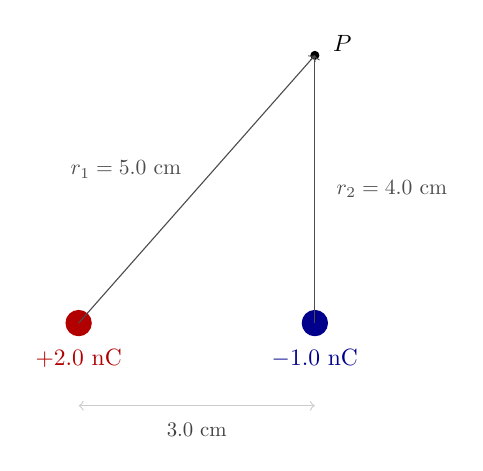
\begin{tikzpicture}[x=1cm,y=1cm]
  \coordinate (Pp) at (1.5,3.4);
  \filldraw[red!70!black] (-1.5,0) circle (0.16);
  \node[red!70!black, scale=0.85] at (-1.5,-0.45) {$+2.0$ nC};
  \filldraw[blue!55!black] (1.5,0) circle (0.16);
  \node[blue!55!black, scale=0.85] at (1.5,-0.45) {$-1.0$ nC};
  \filldraw[black] (Pp) circle (0.05);
  \node[scale=0.85] at (1.85,3.55) {$P$};
  \draw[gray!60!black, ->] (-1.5,0) -- (Pp);
  \node[gray!60!black, scale=0.78] at (-0.9,1.95) {$r_1=5.0$ cm};
  \draw[gray!60!black, ->] (1.5,0) -- (Pp);
  \node[gray!60!black, scale=0.78, anchor=west] at (1.68,1.7) {$r_2=4.0$ cm};
  \draw[gray!40, <->] (-1.5,-1.05) -- (1.5,-1.05);
  \node[gray!50!black, scale=0.75] at (0,-1.35) {$3.0$ cm};
\end{tikzpicture}
\end{center}

The potential is a \emph{scalar} --- no angles, no components. Just add the
two numbers:

\[
V = V_1 + V_2 = \dfrac{1}{4\pi\varepsilon_0}\dfrac{q_1}{r_1}
+ \dfrac{1}{4\pi\varepsilon_0}\dfrac{q_2}{r_2}
\]

\[
V_1 = \ANS{(8.99\times10^9)\dfrac{2.0\times10^{-9}}{0.050} \approx +360\text{ V}}
\qquad
V_2 = \ANS{(8.99\times10^9)\dfrac{-1.0\times10^{-9}}{0.040} \approx -225\text{ V}}
\]

\[
V = \ANS{+360 - 225 = +135\text{ V}}
\]

\checkpoint{Suppose you needed $\vec E$ at $P$ instead of $V$. Would this
same ``just add the numbers'' shortcut work?}

{\small\color{accent} No --- $\vec E$ is a vector, so adding the two
charges' fields needs their directions (components or angles), not just
magnitudes. That's the entire payoff of working with $V$ instead of $\vec
E$ whenever you only need energy: no geometry to track.}

\end{document}
